\documentclass[UTF8, 11pt, oneside]{ctexart}

\usepackage{geometry}
\geometry{a4paper,left=2cm,right=2cm,top=2cm,bottom=1cm}

\usepackage{graphicx}

\usepackage{hyperref}
\hypersetup{colorlinks=true, linkcolor=red}

\linespread{1.6}

\newcommand{\zd}[1]{\textbf{\textcolor[RGB]{123,12,0}{#1}}} % 重点

\def\articletitle{母弱出商贾,父强做侍郎,族望留原籍,家贫走他乡}

\usepackage{fancyhdr}
\usepackage{ifthen}
\pagestyle{fancy}
\fancyhf{}
\setlength{\headheight}{14pt}
\fancyhead[R]{\ifthenelse{\value{page}>1}{\thepage}{}}
\fancyhead[C]{\ifthenelse{\value{page}>1}{\articletitle}{}}
\renewcommand\headrulewidth{0pt}

\usepackage{tcolorbox}
\tcbuselibrary{skins}

\begin{document}

\begin{center}
    \LARGE{\articletitle\footnotemark}
\end{center}
\footnotetext{
    原文出自公众号“远方青木”的文章 《\href{https://mp.weixin.qq.com/s/e740S9DNurMgL2wIFPQe8A}{\articletitle}》
}

我们是该考编入国企,还是在私企拼搏甚至去创业?

我们是该留在老家发展,还是去大城市闯一闯?

今天给大家分享施耐庵在七百年前总结出的一句话:

\begin{tcolorbox}[enhanced,
    frame hidden, interior hidden,
    before skip = 5mm, left skip=10mm,
    borderline west={5pt}{0pt}{blue!50}]
    \zd{母弱出商贾,父强做侍郎,族望留原籍,家贫走他乡。}
\end{tcolorbox}

施耐庵说的是什么意思呢?

先来名词解释,书上给的文言文翻译那种。

首先,母弱和父强是互词,双方是共用的,并不是指母亲弱父亲强,而是指父母弱和父母强。

\zd{母弱出商贾,父强做侍郎的意思,是施耐庵建议后辈如果父母很弱,那就去经商,如果父母很强,那就去做官。}

古代和现代不同,现代商人的地位还可以,但古代讲究的是士农工商,商人地位最低,比农民和工人还低。

为什么父母弱就要去经商,父母弱不应该去务农或者务工么?

因为施耐庵讲的是如何让你走向成功,务农和务工很稳定,但基本不会成功。

\zd{在古代虽然商人地位最低,风险也最大,但对应的是回报也最高,是母弱家庭唯一可能成功的出路。}

那母弱家庭为什么不能直接读书去做侍郎?

因为在古代官的地位是最高的,经济回报也极高,升官发财这个词完美诠释了在古代做官可以名利双收的好生活,士农工商里面士排绝对第一。

\zd{待遇那么好,风险也不大,那自然门槛极高,不然人人都是官了,各种隐形的潜规则也是一道一道的。}

如果母弱,父母没有做过官,那即便你读书天赋好侥幸入了官场,等学会各种官场规则也已经白头,因为这些东西除了你爹妈根本不可能有人会真心教你。

所以在古代,母弱家庭直接冲击官场门槛是事倍功半的一件事,很难取得什么大成就。

\zd{因此,施耐庵建议母弱家庭先经商,成为优秀的商贾,积攒大量钱财后培养后代读书,让后代从小官小吏做起,慢慢摸索规则并传承,一步步向上爬,等到足以称之为父强家庭的时候,再去冲击侍郎之位。}

现代社会的阶级鸿沟没有古代那么夸张,官的地位远没古代那么优越,而商人的地位也远没古代那么低下。

但由于工和农都是稳定生活的代表,厮杀没有那么剧烈,失败的代价小,所以也几乎不存在向上突破的可能。

所以现代社会还是只有官和商才能突破阶层,也还是只有它们才能作为对比。

\zd{官商的差距和古代相比大大缩小,但依然大致符合母弱出商贾,父强做侍郎的规则。}

因此,我们是该考编入国企,还是在私企拼搏甚至去创业这个问题就可以回答了。

\zd{如果你的原生家庭很弱,无法成为你可以依靠的参天大树,那你就去私企拼搏,在商海里厮杀,积累经验和眼界,跟着老板摸爬滚打,如果确定自己是经商那块料,那就试着去创业,这是你能阶层晋升的最大概率途径。}

\zd{如果你的原生家庭很强,是你可以依靠的参天大树,不管这个强指的是商海强还是做官强,那你都应该考编或者入国企,在体制内积累。}

\zd{除非你能确认自己的经商天赋已经逆天到足以撼动原生家庭,否则考编入国企一定是你的最佳选择。}

\zd{父越强,你的天赋能撼动原生家庭的概率就越低,你选择经商搏一把就越不划算。}

举个例子,王思聪,他爹积累下千亿财富后原生家庭过于强大,以至于只要王思聪选择创业搏一把那基本就是注定错误的,除非他是亿中无一的天才,这概率实在是太低了。

但他如果老老实实考编入国企,哪怕只是当个科长处长,那他也是正确的,至少是上进的。

当然现在都是独生子,没那么多孩子可以四处铺路,只有一个孩子的话那王思聪就一条路,继承家业,做到这一点就是上进的好孩子,这是他爹唯一希望他走的路。

但如果王思聪不愿意继承家业,那父强家庭的他,考编远强于创业,因为考编慢慢爬仕途别人都不会说你错,而创业就几乎注定了别人最后会说你错。

如果王健林有多个孩子,那么留一个继承家业,其他都安排去走仕途才是对王家来说的最优选择。

\zd{那什么叫族望留原籍,家贫走他乡?}

这里涉及到一个家族或者说宗族的概念,现代中国经历过剧烈的改革,宗族几乎彻底解体,而由于独生子女政策连家族都大大衰弱。

但全球除中国之外的其他国家,以及古代的中国,家族和宗族的概念都是极为兴盛的。

血亲具有天然的信任关系,双方天然相信对方可以和自己互帮互助,对血亲给与的无偿帮助,我们无条件相信对方愿意在十年二十年之后,会以其他形式偿还过来,这是对陌生人来说不可能的事情。

所以血亲之间能展开的合作种类和范围极多,而陌生人之间基本只相信钱,交易都是实时完成的,不存在先款,十年后再收货这种可能性。

绝大多数中国人从未体验过家族和宗族的感觉,只有小时候回老家才能感受那老家人极其亲切的态度。

但从全世界规律来看,中国这种家族和宗族的消失是暂时的,长久来看必定回归,无非是规模和强度没有古代那么大了而已,但性质是一样的。

\zd{在古代,施耐庵教导后辈族望留原籍,家贫走他乡。}

\zd{意思就是如果你出生于名门望族,家族强大,宗族强大,那你就尽量留家族和宗族的所在地生活和工作。}

\zd{反过来,如果你的家族衰弱,宗族衰弱,那你就尽量远走他乡,不要留在原籍。}

族望留原籍的道理很简单,在人生的起步阶段一个人需要的帮助是多维度的,其中很多帮助都是无法用钱购买的,而年轻人需要的很多帮助也不能立刻给予对方回报,很多只能在十年二十年之后以其他各种形式给予回馈。

那这种帮助除了血亲,是不可能有人愿意帮你的,在宗族内这个叫人情往来。

因此,如果你族旺,那么留原籍对你会有极大的帮助,可以让你迅速渡过起步阶段,人生之路和别人相比顺风顺水的多。

即便你的宗族在小县城,那么生活也会比那些在北上广打拼的人舒服的多。

\begin{figure*}[htbp]
    \centering
    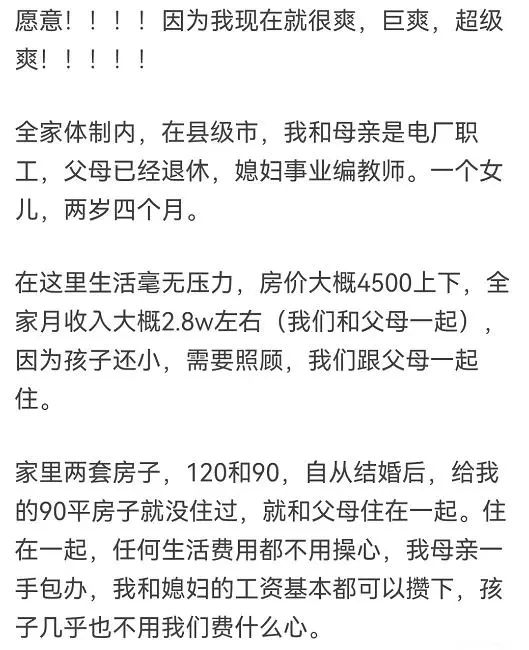
\includegraphics[width=10cm]{2023-01-07-001.jpg}
\end{figure*}

\zd{上面贴的这个根本不能称之为宗族,在家族里面也不算兴旺的,只能说父母过的还算行,在当地也就算个中产家庭偏上,要是在北上广他父母积累的那点财富啥都不算。}

\zd{即便这样,他回原籍工作,生活的也巨幸福,人生巨爽。}

要是那种参天大树般的古代宗族,而你恰好又出生在这种宗族,那肯定回原籍发展才是最好选择。

\zd{但如果你的家族不行,宗族不行,那施耐庵就不建议你留原籍了,而是建议你家贫走他乡。}

因为家族和宗族都不行的话,那你留原籍发展人生的起步阶段就没人能帮你,你能依靠的只有自己。

而你的家族和宗族在当地都不行,不管什么原因,那自然是有原因的,你继续留原籍工作能出人头地的概率也会很低。

既然如此,不如远走他乡闯一闯。

\zd{去他乡闯荡无依无靠,如无根浮萍,起步阶段远弱于本地人,但没关系,因为在老家自己也是无宗族之人,也是无依无靠如无根浮萍,双方没有本质区别。}

\zd{既然如此,那我当然要去更富有发展机会的地方闯一闯,哪里适合自己去哪里,不必刻意把自己死死的限定在原籍。}

现代中国宗族彻底消失,只有极少数人还有微弱的家族,其余绝大多数中国人实际上能依靠的只有自己,父母能给与的帮助都不多,换句话说几乎所有人都符合家贫走他乡的定义。

于是现代中国发生了人类有史以来最大的迁移潮,大家都往大城市涌,因为大城市机会最多,翻身的概率最大。

反正自己没有家族和宗族能帮忙,老家对自己毫无吸引力,如果什么都要靠自己,那为什么不来大城市试一试?

于是大家都家贫走他乡,只有极少数能享受到家族帮助的人才愿意主动留原籍。

全球其他国家多多少少都有家族和宗族的存在,愿意留原籍的人还是很多的,而人口慢慢向大城市转移后,很多定居之人的原籍就变成了大城市,然后慢慢把家族之人接过来一起定居,于是没有发生中国那么离谱的春运迁移潮。

但随着时间的积累,中国早晚也会和其他国家一样的,当然由于生育率的暴跌,宗族想复原那几乎是不可能了,就连兴旺的家族也会很少有,绝大多数家族里未来也只会是大猫小猫两三只。

但就算是这样的迷你家族,如果在原籍扎根够深,也能给与很大帮助。

再过几十年,大家慢慢都在城市定居后,到时候愿意背井离乡去外地拼搏的中国人会越来越少,愿意留原籍的人会越来越多。

那现在就可以回答上面写的第二个问题了,我们是该留在老家发展,还是去大城市闯一闯?

\zd{很简单,看看自己的家族是否够强大,是否符合族望留原籍的标准。}

\zd{如果家族够兴旺,符合这个标准,那就留老家发展,去大城市闯反而浪费了自身优势,因为家中父兄完全没办法帮你。}

如果家族啥都没有,啥帮助都不能给你,那当然要去大城市闯一闯,努力拼搏一下看能否扎根大城市,如果扎根了以后大城市就是你孩子的原籍,他就不用操心是留老家发展还是大城市闯一闯这个问题了。

\zd{母弱出商贾,父强做侍郎,族望留原籍,家贫走他乡,你很多人生问题的答案其实都浓缩在这句话中。}

\zd{这是施耐庵七百年前留给我们中国人的宝贵文化遗产。}

\end{document}

